\section{Correspondende of the two definitions}
In this first section the pseudospectrum of a \texttt{grcar} matrix will be computed in two different ways. \texttt{Grcar} is an n-by-n Toeplitz matrix with -1s on the subdiagonal, 1s on the diagonal, and 3 superdiagonals of 1s.\footnote{Matlab documentation of the gallery command.} In order to compute the pseudospectrum it is helpful to reformulate the definition of the pseudosprectrum
\begin{align}
\| (z\mathbf{I} - \mathbf{A})^{-1} \|_2 > \epsilon^{-1} & \;\;\;\;\;\;\;\; \mathbf{B} = z\mathbf{I} - \mathbf{A}      \\
\| (\mathbf{B})^{-1} \|_2 > \epsilon^{-1}               & \;\;\;\;\;\;\;\; \mathbf{B} = \mathbf{U} \Sigma \mathbf{V}  \\
\| (\mathbf{U} \Sigma \mathbf{V})^{-1} \|_2 > \epsilon^{-1} \\
\| (\mathbf{U} \Sigma^{-1} \mathbf{V}) \|_2 > \epsilon^{-1} & \;\;\;\;\;\;\;\; \text{$\sigma_{min}$ is the largest $\sigma$ of $\Sigma^{-1}$}  \\
\sigma_{min}^{-1} > \epsilon^{-1} \\
\sigma_{min}(z\mathbf{I} - \mathbf{A}) < \epsilon \\
\end{align}
here $sigma$ stands for the set of singular values. A point $z$ is thus contained in the Pseudospectrum, if the smallest singular value of $z\mathbf{I} - \mathbf{A}$ is smaller then $\epsilon$. Using the definition above the pseudospectrum $\Lambda_\epsilon$ can be simply be computed on a grid by running.\footnote{Trefethen Embree, Spectra and Pseudospectra page 372.}
\begin{lstlisting}[language = matlab]
	m = length(x);
	m2 = length(y);	

	for k=1:1:m, for j =1:1:m2
		sigmin(j,k) = min(svd((x(k)+y(j)*i)*eye(N)-A));
	end, end
	contour(x,y,-log10(sigmin1))
\end{lstlisting}
The code snipped above has been used to compute the pseudospectrum shown in figure~\ref{fig:pseudoGrcar}. With \texttt{N = 63} and \texttt{A = gallery('grcar',N)}, \texttt{x} and \texttt{y} define the vectors along the axes. 
\begin{figure}
\centering
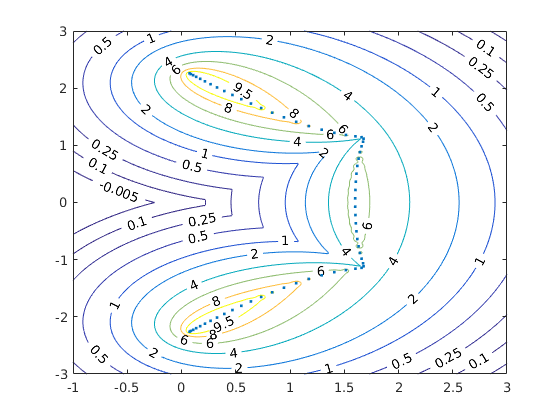
\includegraphics[width=0.7\linewidth]{../src/figures/grcar}
\caption{Plot of the Pseudospectrum of the \texttt{grcar matrix}.}
\label{fig:pseudoGrcar}
\end{figure}

The pseudospectrum can also be defined trough random perturbations using 
\begin{equation}
 z \in \Lambda(\mathbf{A} + \mathbf{E}) \;\; \text{with} \; \mathbf{E} \in \mathbb{C}^{n,n} \; \text{and} \|\mathbf{E}\| < \epsilon.
\end{equation}

\begin{figure}
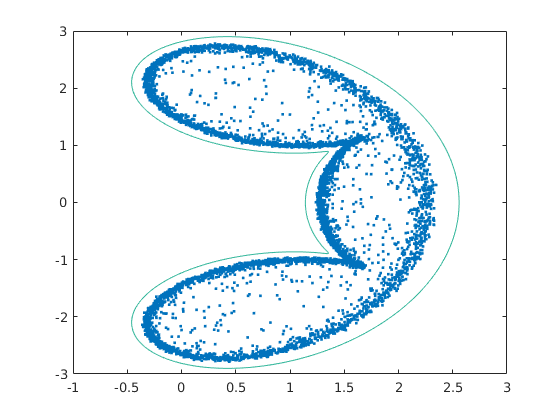
\includegraphics[width=0.5\linewidth]{../src/figures/randPert}
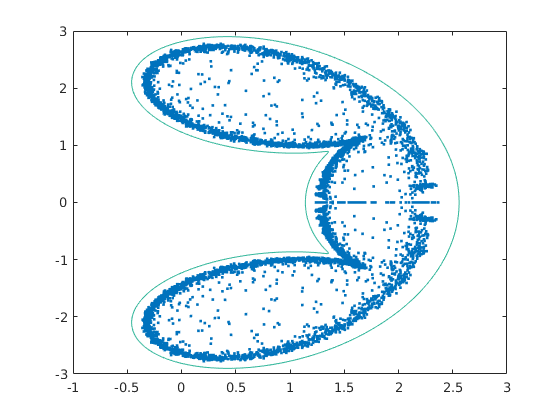
\includegraphics[width=0.5\linewidth]{../src/figures/randPertReal}
\caption{Plot of the $\epsilon = 0.1$ and perturbed eigenvalues. }
\label{fig:randPerts}
\end{figure}
